\documentclass[20pt]{report}
\usepackage{graphicx} % Required for inserting images
\usepackage[T1]{fontenc} % Lettere accentate da tastiera
\usepackage[English]{babel} % Lingua del documento
\usepackage{lipsum} % Genera testo fittizio
\usepackage{amsmath,amssymb} % Per formule
\usepackage[a4paper, total={6in, 8.3in}]{geometry}
\usepackage{siunitx}
\usepackage{hyperref}
\usepackage{array} % Per modificare lo spazio tra le righe della tabella
\usepackage{adjustbox} % Pacchetto per regolazioni avanzate
\usepackage{float}
\usepackage{overpic}
\usepackage[absolute,overlay]{textpos} % Per posizionare il testo o le immagini in modo preciso
\usepackage{hyperref}
\usepackage{media9}





\title{Assignments}
\author{Filippi Matteo\\Firmani Daniele\\Galenda Andrea\\Gorla Alessandro}
\date{}

\begin{document}

% Inizio copertina
\begin{titlepage}
    \centering
    

    \begin{flushleft}
    
    
\includegraphics[scale=0.07]{Images/LogoPolimi.jpg}\par\vspace{1cm}

    \vspace*{0.5cm}
    
    \huge
    \textbf{Advanced Dynamics of Mechanical Systems}\\ 
    \vspace*{0.5cm}
    \Large
    
    \end{flushleft}
    
    \Large
    
    \vspace{2.5cm}
    
    \begin{flushright}
    Authors:\\
    \vspace{0.1cm}
    Andrea GALENDA\\Matteo FILIPPI\\Daniele FIRMANI\\Alessandro GORLA
    %\textbf{Matteo FILIPPI\\Daniele FIRMANI\\Andrea GALENDA\\Alessandro GORLA}
    \end{flushright}

    \vspace{0.4cm}
    
    \begin{flushleft}
        \Large
        Professor: \par
        \vspace{0.1cm}
        Prof. Stefano MELZI\par
        \vspace{0.5cm}
        Teaching Assistant: \par
        \vspace{0.1cm}
        Giulia POMARANZI\par
    \end{flushleft}
    \vfill
    {\Large Academic Year 2023/2024\par}
    
\end{titlepage}
% Fine copertina

\newpage
% Creare una pagina vuota
\thispagestyle{empty} % Evita l'inserimento di intestazioni o piedini
\mbox{} % Inserisce uno spazio vuoto per creare una pagina vuota
\newpage

% Sommario senza numero di pagina
\tableofcontents
\thispagestyle{empty}

\newpage

% Resetta la numerazione delle pagine
\pagenumbering{arabic}


\addcontentsline{toc}{part}{Modal Analysis}
\part*{Modal Analysis}


\newpage

\chapter*{Cantilever Beam}
\addcontentsline{toc}{chapter}{Cantilever Beam}

\setcounter{page}{2}
\pagestyle{plain}

\renewcommand{\thesection}{\arabic{section}} % Utilizza numerazione 1, 2, 3 invece di 0.1, 0.2, 0.3


\section{Introduction}
The objective of this first part is to derive the natural frequencies and the mode shapes of the structure.\\ 
The second part consists of carrying out a modal parameters identification procedure starting from the structure frequency response functions.\\
The FRFs are computed analytically (for assigned input and output positions) from the mathematical model, but they're then considered as representative of an experimental test.\\
The modal parameters identification is carried out according to the FRF-based multi-mode curve fitting method.\\

\section{Analytical model}
The structure under analysis is a cantilever beam characterised by the following geometric and structural properties.

\begin{figure}[H]
    \centering
    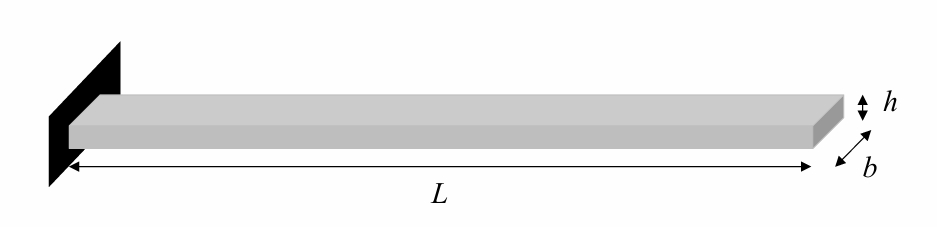
\includegraphics[scale=0.35]{Images/Cantilever.jpeg}
\end{figure}

\begin{table}[h]
\centering
\renewcommand{\arraystretch}{1.4} % Imposta lo spazio tra le righe della tabella
\setlength{\tabcolsep}{13pt} % Imposta lo spazio tra le colonne della tabella
\begin{tabular}{|l|c|c|c|}
\hline
\textbf{Parameter}      & \textbf{Symbol} & \textbf{Unit}  & \textbf{Value} \\ \hline
Length                  & \(L\)           & mm             & 1200           \\ \hline
Thickness               & \(h\)           & mm             & 8              \\ \hline
Width                   & \(b\)           & mm             & 40             \\ \hline
Density                 & \(\rho\)        & \si{kg/m^3}    & 2700           \\ \hline
Young's Modulus         & \(E\)           & GPa            & 68             \\ \hline
\end{tabular}
\caption{Geometrical and structural properties of the beam}
\label{table:beam_parameters}
\end{table}


\subsection{Boundary conditions}
Starting from the cantilever beam standing wave solution:
\begin{equation*}
    w(x,t)=\left[A cos(\gamma x) + B sin(\gamma x) + C cosh(\gamma x) + D sinh(\gamma x)\right] cos(\omega t + \phi )
\end{equation*}
constants A, B, C and D can be computed by applying 4 BCs.\\
Indeed knowing vertical displacement and rotation at the clamped section (both are null), and applying moment equilibrium and vertical force equilibrium at the free end of the beam, four equations in four unknowns can be written:
\begin{equation}
    w(0,t)=0 \ \ \ \ \forall t
\end{equation}
\begin{equation}
     w'(0,t)=0 \ \ \ \ \forall t
\end{equation}
\begin{equation}
     E J w''(L,t)=0 \ \ \ \ \forall t 
\end{equation}
\begin{equation}
     E J w'''(L,t)=0 \ \ \ \ \forall t
\end{equation}
These 4 equations can be rewritten in a matrix way as in the following:
\begin{equation*}
    \begin{bmatrix}
    1 & 0 & 1 & 0 \\
    0 & 1 & 0 & 1 \\
    -cos(\gamma L) & -sin(\gamma L) & cosh(\gamma L) & sinh(\gamma L) \\
    sin(\gamma L) & -cos(\gamma L) & sinh(\gamma L) & cosh(\gamma L)
    \end{bmatrix}
    \begin{Bmatrix}
    A \\ B \\ C \\ D
    \end{Bmatrix}
    = \underline 0
\end{equation*}
Or equivalently:

\begin{equation*}
[H(\omega )]\underline z = \underline 0
\end{equation*}

\subsection{Natural frequencies and mode shapes computation}

Now it's possible to compute the eigenfrequencies of the structure by numerically solving the following equation: \(\det([H(\omega)]) = 0\)\\
Then, the shape functions can be simply computed substituting the obtained eigenfrequencies into the following equation:
\begin{equation*}
    \phi(x)=A cos(\gamma x) + B sin(\gamma x) + C cosh(\gamma x) + D sinh(\gamma x)
\end{equation*}
By following this procedure, the following results have been obtained: 

\begin{figure}[H]
    \centering
    \makebox[\textwidth]{\hspace{-1.6cm} % Sposta tutto di 2cm a destra, usa valori negativi per spostare a sinistra
        \begin{minipage}{0.4\textwidth}
            \centering
            \begin{tabular}{c|c}
            \multicolumn{1}{c}{\textbf{Mode}} & \multicolumn{1}{c}{\textbf{Natural frequency [Hz]}}\\
                1 & 4.50 \\
                2 & 28.22 \\
                3 & 79.03 \\
                4 & 154.87 \\
            \end{tabular}
        \end{minipage}
        \hspace{0.04\textwidth} % Spazio tra tabella e immagine
        \begin{minipage}{0.45\textwidth}
            \centering
            \phantomsection\label{fig:modeshapes} % Ancora invisibile per l'immagine
            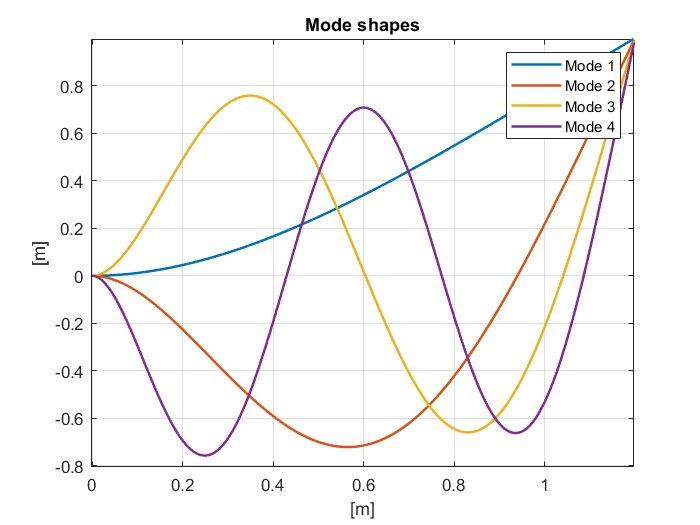
\includegraphics[scale=0.37]{Images/Modeshapes.jpg}
        \end{minipage}
    } 
    \caption{Eigenfrequencies and mode shapes of the structure}
    \label{fig:modeshapes-caption}
\end{figure}
\newpage
\section{Modal parameters identification}

This second part consists in computing the FRFs for four different pairs of input and output positions.\\
Once we have these curves we assume them to be representative of the results of an experimental test performed on our structure.\\
Starting from this experimental FRFs we carry out a modal parameters identification procedure in order to derive the eigenfrequencies and the mode shapes of the structure

\subsection{Calculation of the FRFs}

 For the analytical computation of the FRFs, four pairs of input ($x_k$) and output ($x_j$) positions are chosen, as shown in \hyperref[experimental FRFs]{Figure 2}.\\
 The FRFs have been computed trhough the following equation:
\begin{equation*}
G_{jk}(\Omega) = \sum_{i=1}^{n} \frac{\Phi_i(x_j) \Phi_i(x_k) / m_i}{-\Omega^2 + j 2 \xi_i \omega_i \Omega + \omega_i^2}
\end{equation*}
The non dimenional damping ratio is assumed equal to 1\%, while modal masses are computed as:
\begin{equation*}
    m_i=\int_{0}^{L}m\Phi_i^2(x)dx
\end{equation*}
The resulting four FRFs are here represented both in terms of module and phase:
\begin{figure}[H]
    \centering
    \phantomsection\label{experimental FRFs} % Ancora invisibile per l'immagine
    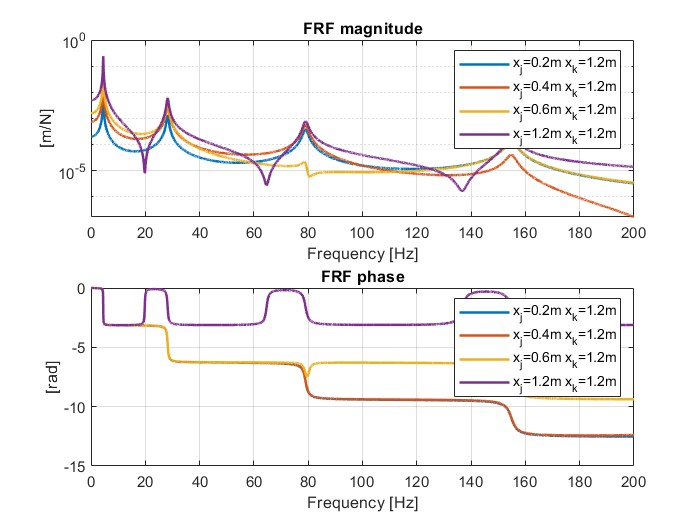
\includegraphics[scale=0.5]{Images/FRFExp.jpg}
    \caption{FRFs of the different four pairs of input and output positions}
\end{figure}
\newpage
\subsection{FRFs fitting}
As previously said, the FRFs above are from now on considered to be extracted from experimental tests on the structure.\\
Indeed, the aim is to obtain numerical FRFs computed through the best fitting method:
\begin{equation*}
    G_{jk}^{NUM}(\Omega)=\sum_{i=1}^{n}\frac{A_{jk}^{(i)}}{-\Omega^2+j2\xi_i\omega_i\Omega+\omega_i^2}+\frac{R_{jk}^L}{\Omega^2}+R_{jk}^H
\end{equation*}
Modal parameters of the new FRFs are extracted from a minimization of the following error function:
\begin{equation*}
    \epsilon=\sum_{r=1}^{N}\sum_{s=1}^{M}Re(G_r^{EXP}(\Omega_s)-G_r^{NUM}(\Omega_s))^2+Im(G_r^{EXP}(\Omega_s)-G_r^{NUM}(\Omega_s))^2
\end{equation*}
Starting from a vector of initial guesses the error minimisation procedure has been carried out by using 
\texttt{lsqnonlin} Matlab function.\\ 
For each natural frequency a range of 5 Hz has been considered.\\\\
The results of the fitting operations are reported below:
\begin{figure}[H]
    \centering
    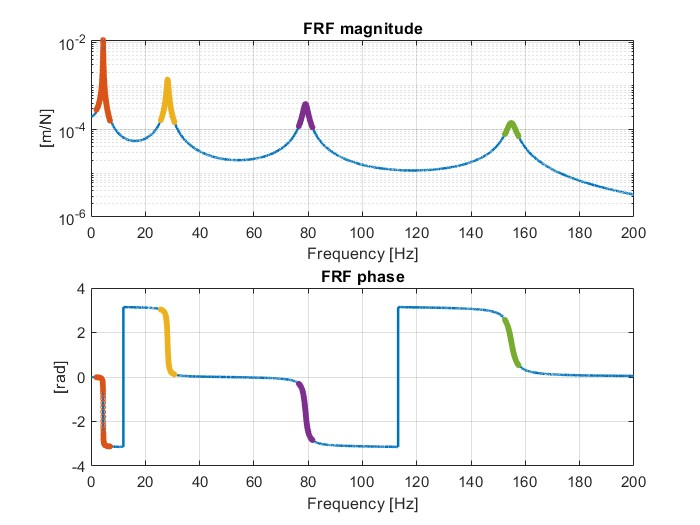
\includegraphics[scale=0.5]{Images/0_2.jpg}
    \caption{Fitting results for \(x_j = 0.2\;\text{m}\) and \(x_k = 1.2\;\text{m}\)}
\end{figure}
\begin{figure}[H]
    \centering
    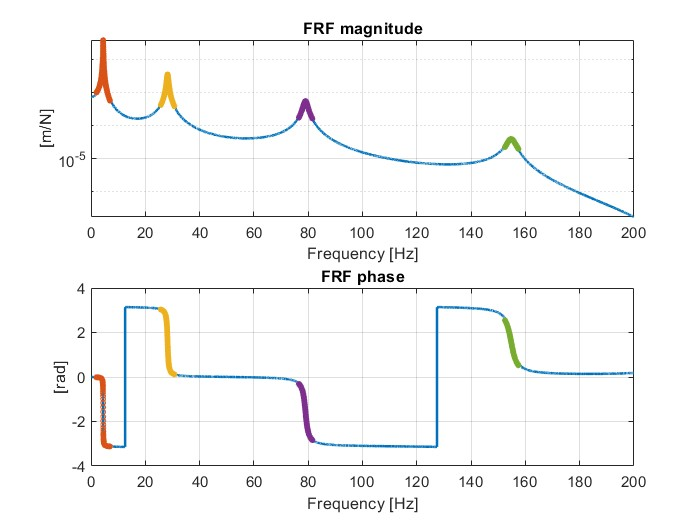
\includegraphics[scale=0.5]{Images/0_4.jpg}
    \caption{Fitting results for \(x_j = 0.4\;\text{m}\) and \(x_k = 1.2\;\text{m}\)}
\end{figure}
\begin{figure}[H]
    \centering
    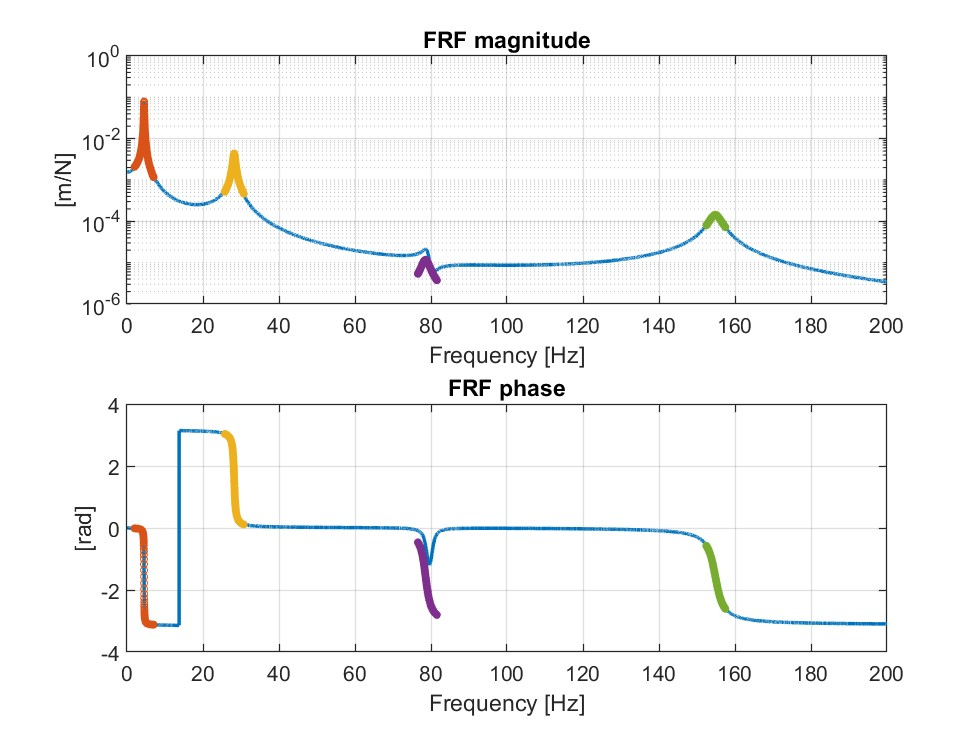
\includegraphics[scale=0.355]{Images/0_6.jpg}
    \caption{Fitting results for \(x_j = 0.6\;\text{m}\) and \(x_k = 1.2\;\text{m}\)}
\end{figure}
\begin{figure}[H]
    \centering
    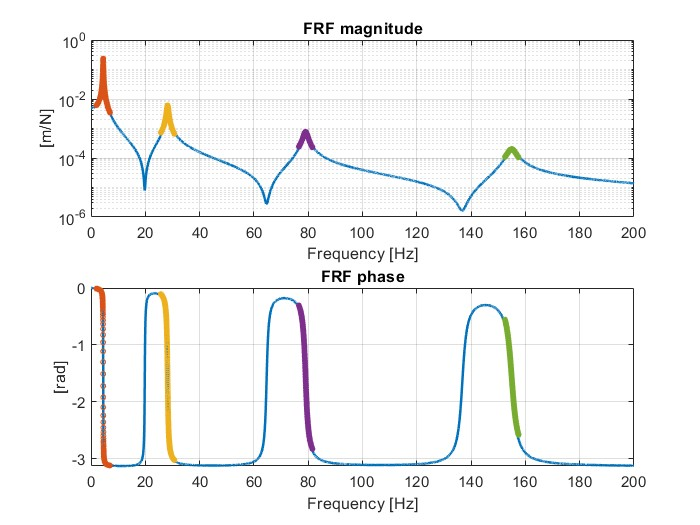
\includegraphics[scale=0.5]{Images/1_2.jpg}
    \caption{Fitting results for \(x_j = 1.2\;\text{m}\) and \(x_k = 1.2\;\text{m}\)}
\end{figure}
\noindent As can be seen in \hyperref[fig:modeshapes]{Figure 1} the third output position (0.6 m) has been chosen in correspondence of a node of the third mode. \\
For such case obvioulsy the fitted FRF is not reliable.

\subsection{Mode shapes reconstruction}
\label{Mode shapes reconstruction}
Starting from the numerical FRFs, obtained through the best fitting method, it has been possible to reconstruct the mode shapes. \\
Obviously the numerical mode shapes are known just in correspondence of the points in which the experimental FRFs have been measured.\\
The value assumed by the reconstructed mode shape \(\phi_i\) in correspondence of the \(j\)-th measuring point \(x_j\), is computed as:\\
\begin{equation*}
\phi_i \left(x_j \right) = - Imag\left( G_{jk} \left(\omega _i \right) \right)
\end{equation*}
The reconstructed mode shapes are reported below.\\
\begin{figure}[H]
    \centering
    \begin{overpic}[scale=0.48]{Images/ReconstructedModes.jpg} % L'immagine di sfondo
        \put(67,10){ % Coordina per posizionare l'immagine sovrapposta, da regolare manualmente
            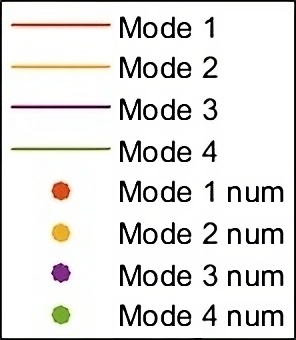
\includegraphics[scale=0.25]{Images/Legenda.png} % L'immagine sovrapposta
        }
    \end{overpic}
    \caption{Reconstructed mode shapes}
    \label{fig:overlay}
\end{figure}

\newpage


\chapter*{Rail Wheel}
\addcontentsline{toc}{chapter}{Rail Wheel}

\newcounter{sectionB}
\setcounter{sectionB}{0}
\renewcommand{\thesection}{\arabic{sectionB}}

\stepcounter{sectionB}
\section{Introduction}
\phantomsection


This second part consists in a modal parameters identification starting from real experimental data coming from vibration measurements of a rail wheel.
\begin{figure}[H]
    \centering
    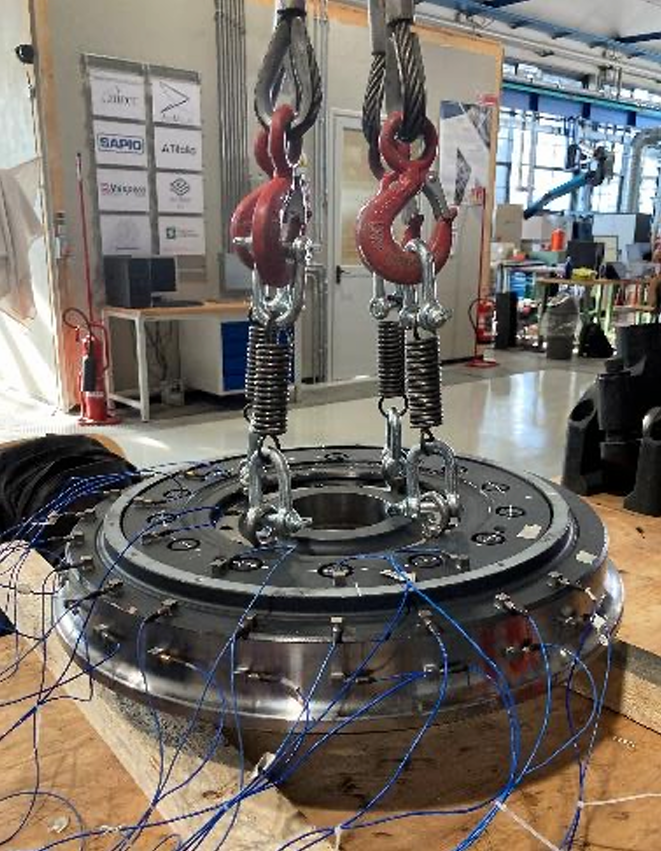
\includegraphics[width=0.5\linewidth]{Images/wheel.png}
    \caption{Experimental setup}
\end{figure}
\noindent
The wheen has been suspended through elastic supports and a dynamo-metric impact hammer has been leveraged to apply an axial load.\\
The output was measured by placing twelve accelerometers on half of the wheel exploiting the symmetry of the structure.\\
The resulting measurements have been used to generate a dataset containing twelve FRFs and their corresponding coherence functions.
\begin{figure}[H]
    \centering
    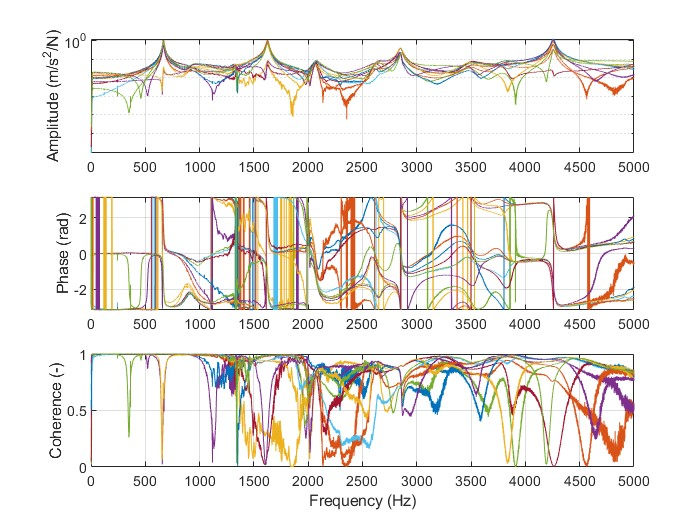
\includegraphics[scale=0.5]{Images/DataParteB.jpg}
    \caption{Experimental FRFs and coherence functions}
\end{figure}

\stepcounter{sectionB}
\section{Modal parameters identification}
\phantomsection

Similarly to the previous section, numerical FRFs have to be computed starting from experimental data, exploiting an error minimisation procedure.
\subsection{Initial guesses estimation}
\phantomsection
Starting from data shown above, initial guesses are computed exactly as before, exception made for the calculation of natural frequencies.\\
Indeed, the first two natural frequencies of each FRF have been computed (these are the only ones of interest in this case), then the ones related to a non reasonable value of the coherence function have been deleted.\\
Finally, a mean of the remaining frequencies has been conducted for each mode. \\
The resulting eigenfrequencies are the following ones:\\
\begin{center}
    \begin{tabular}{c|c}
        \multicolumn{1}{c}{\textbf{Mode}} & \multicolumn{1}{c}{\textbf{Natural frequency [Hz]}}\\
        1 & 667.3 \\
        2 & 1625 \\
    \end{tabular}
\end{center}
\vspace{1 cm}


\subsection{Best fitting procedure}
\phantomsection
Once the initial guesses have been estimated, the minimization procedure can be applied. \\This procedure consists in a comparison between experimental and numerical FRFs; the latter ones computed according to the best fitting method.\\
The fitting results are here reported:
\begin{figure}[H]
    \centering
    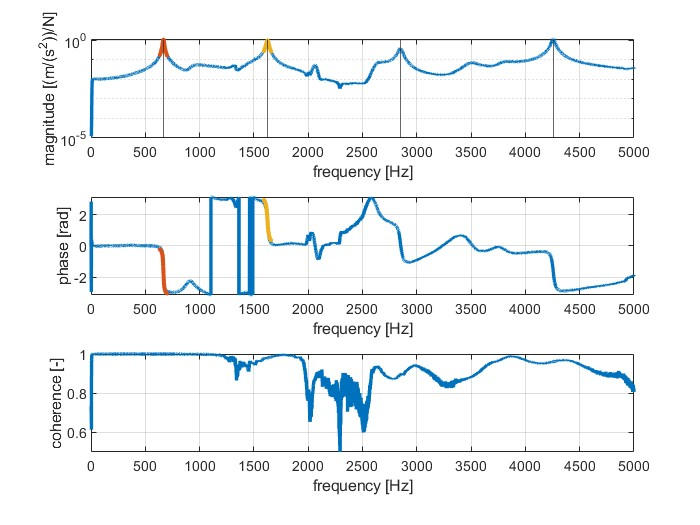
\includegraphics[scale=0.5]{Images/1.jpg}
    \caption{Fitting results of the $1^{\text{st}}$ sensor FRF}
\end{figure}
\begin{figure}[H]
    \centering
    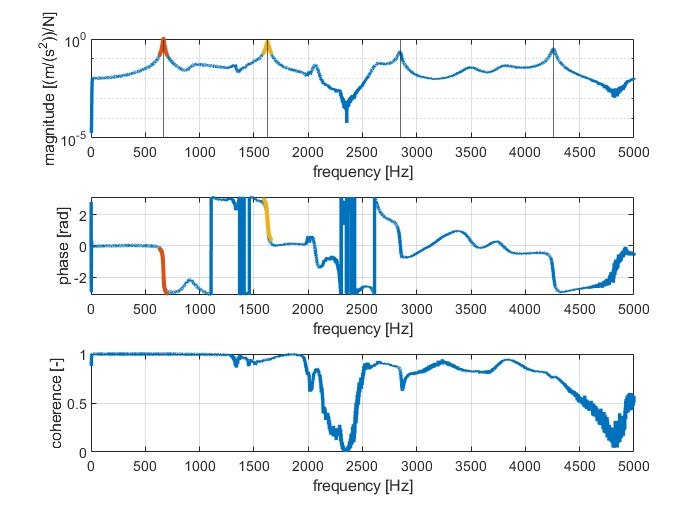
\includegraphics[scale=0.5]{Images/2.jpg}
    \caption{Fitting results of the $2^{\text{nd}}$ sensor FRF}
\end{figure}
\begin{figure}[H]
    \centering
    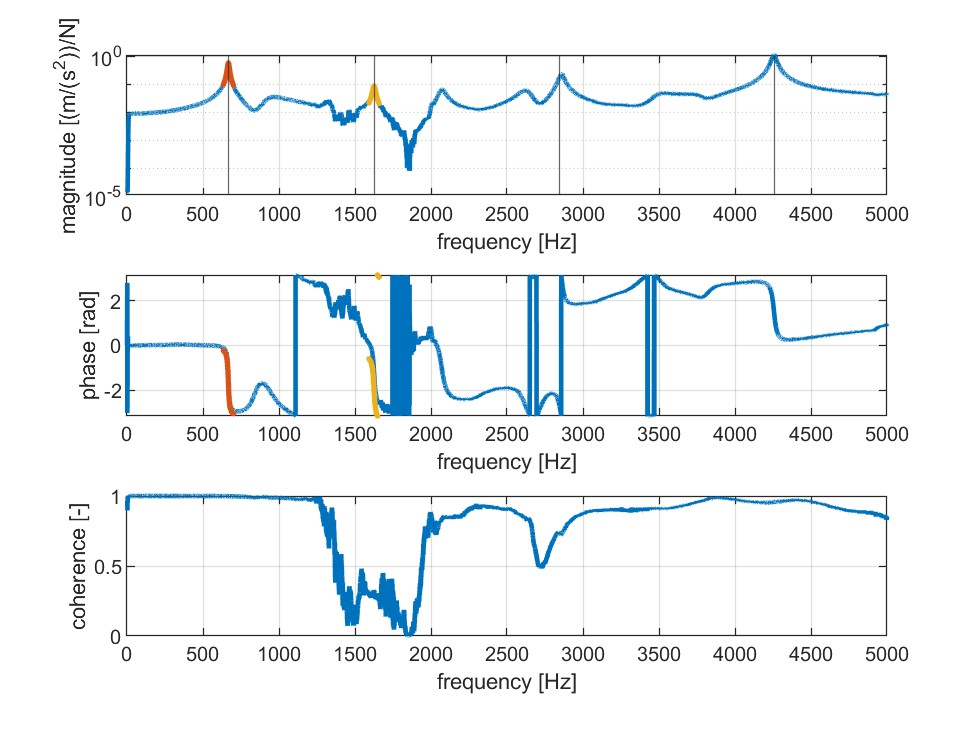
\includegraphics[scale=0.355]{Images/3.jpg}
    \caption{Fitting results of the $3^{\text{rd}}$ sensor FRF}
\end{figure}
\begin{figure}[H]
    \centering
    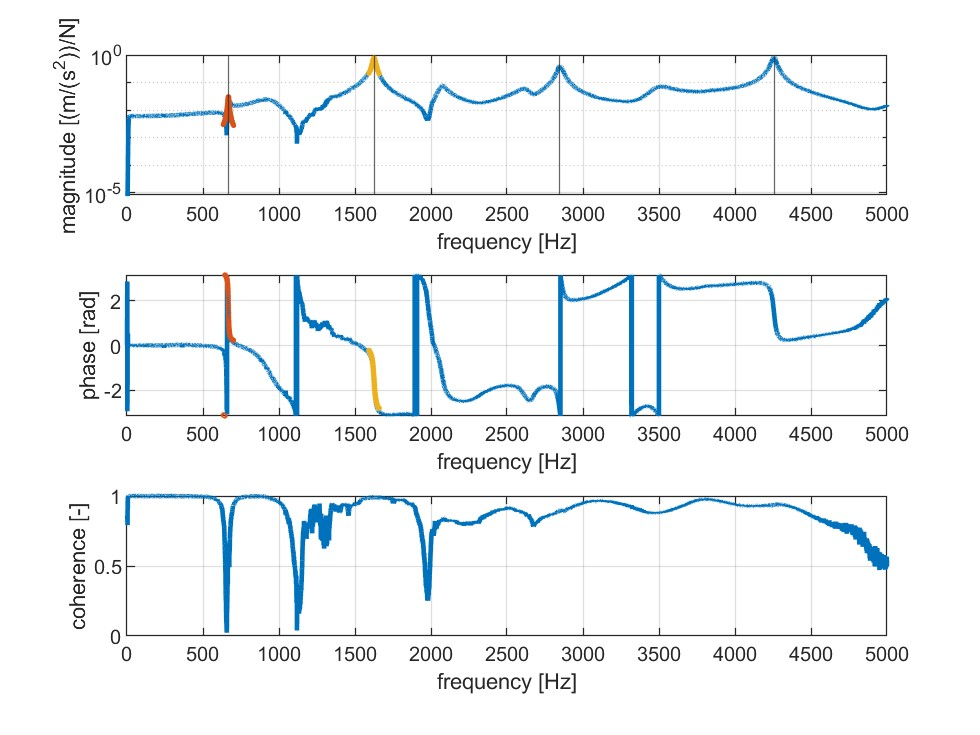
\includegraphics[scale=0.355]{Images/4.jpg}
    \caption{Fitting results of the $4^{\text{th}}$ sensor FRF}
\end{figure}
\begin{figure}[H]
    \centering
    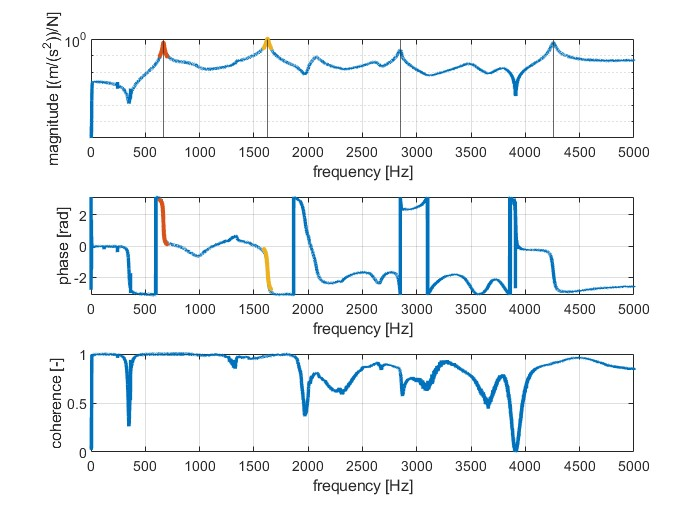
\includegraphics[scale=0.5]{Images/5.jpg}
    \caption{Fitting results of the $5^{\text{th}}$ sensor FRF}
\end{figure}
\begin{figure}[H]
    \centering
    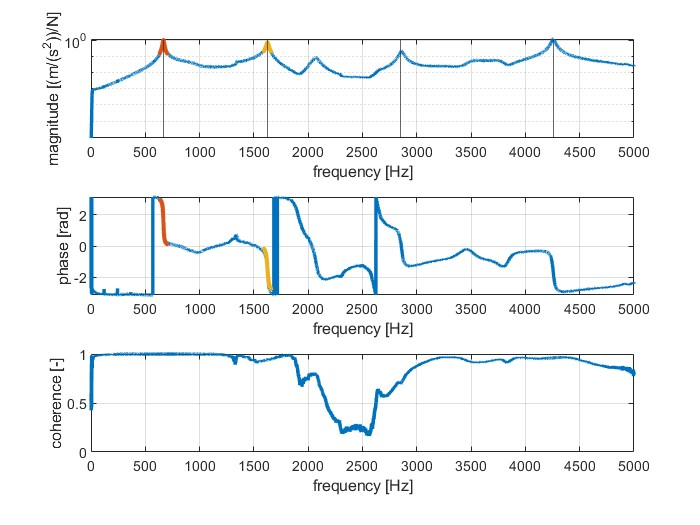
\includegraphics[scale=0.5]{Images/6.jpg}
    \caption{Fitting results of the $6^{\text{th}}$ sensor FRF}
\end{figure}
\begin{figure}[H]
    \centering
    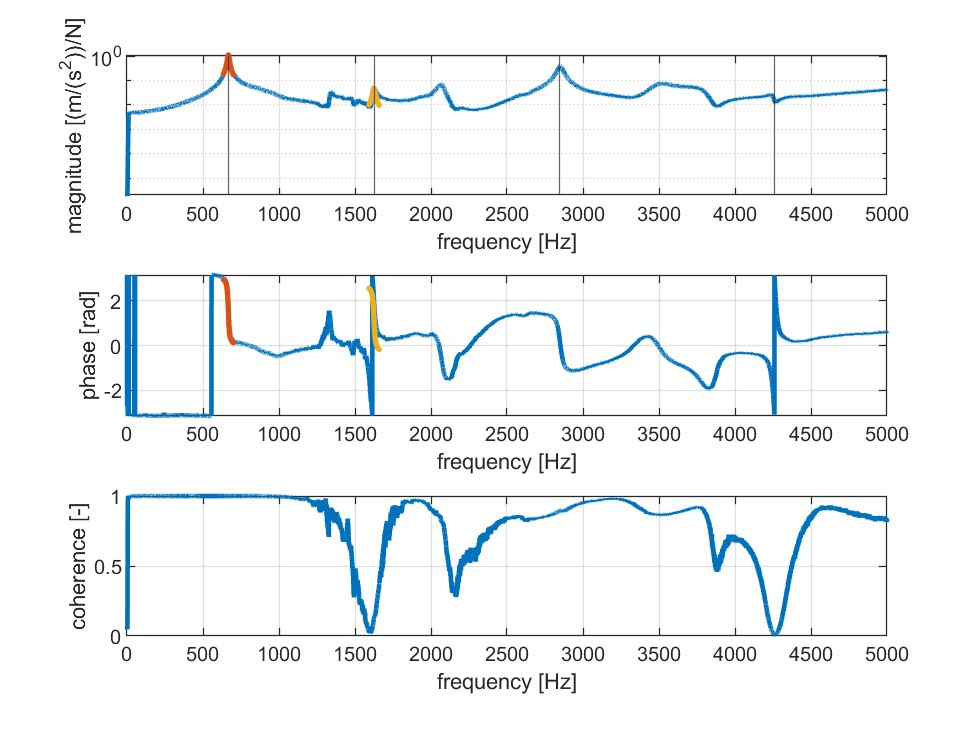
\includegraphics[scale=0.355]{Images/7.jpg}
    \caption{Fitting results of the $7^{\text{th}}$ sensor FRF}
\end{figure}
\begin{figure}[H]
    \centering
    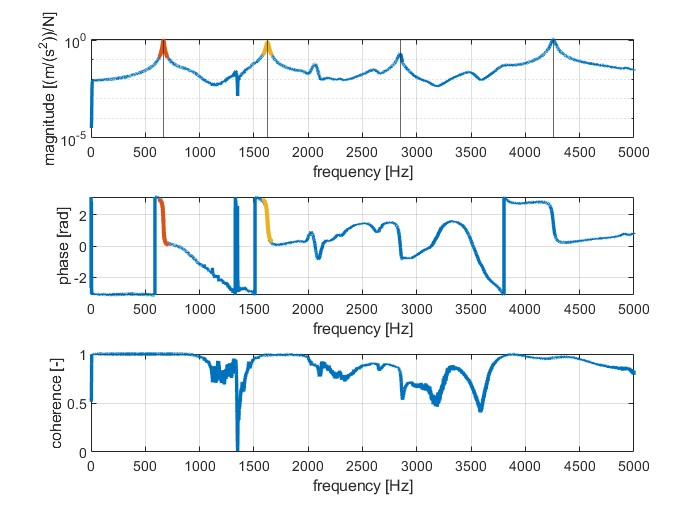
\includegraphics[scale=0.5]{Images/8.jpg}
    \caption{Fitting results of the $8^{\text{th}}$ sensor FRF}
\end{figure}
\begin{figure}[H]
    \centering
    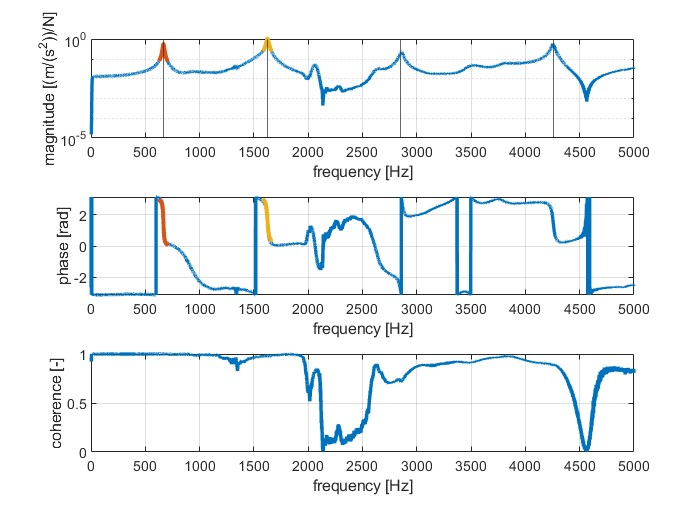
\includegraphics[scale=0.5]{Images/9.jpg}
    \caption{Fitting results of the $9^{\text{th}}$ sensor FRF}
\end{figure}
\begin{figure}[H]
    \centering
    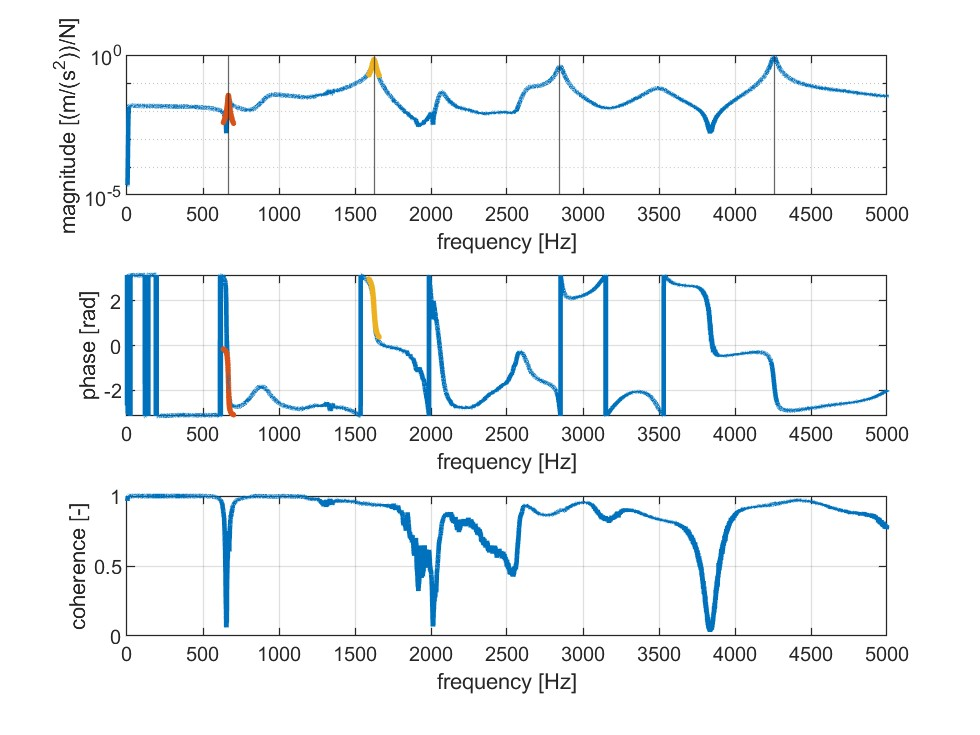
\includegraphics[scale=0.355]{Images/10.jpg}
    \caption{Fitting results of the $10^{\text{th}}$ sensor FRF}
\end{figure}
\begin{figure}[H]
    \centering
    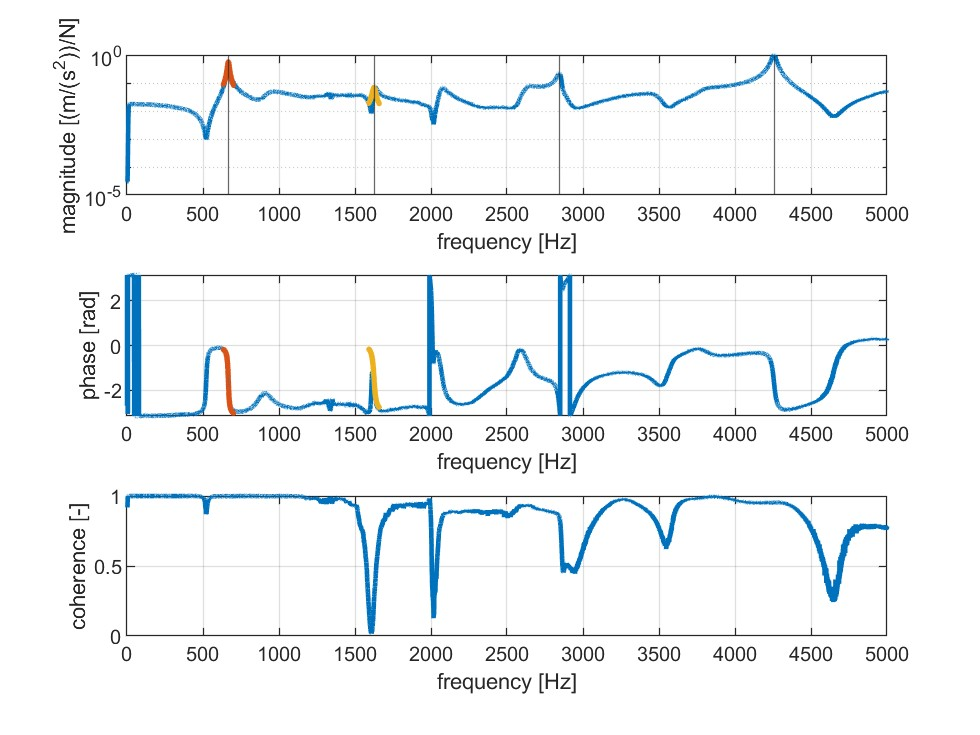
\includegraphics[scale=0.355]{Images/11.jpg}
    \caption{Fitting results of the $11^{\text{th}}$ sensor FRF}
\end{figure}
\begin{figure}[H]
    \centering
    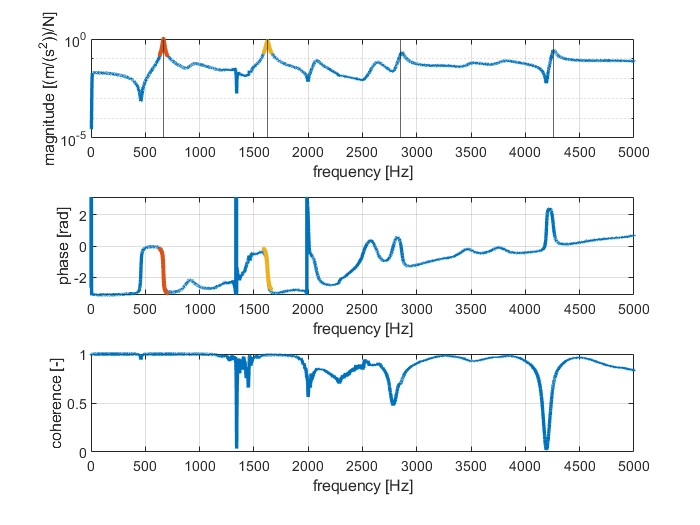
\includegraphics[scale=0.5]{Images/12.jpg}
    \caption{Fitting results of the $12^{\text{th}}$ sensor FRF}
\end{figure}
\noindent In the figures above, it can be seen that whenever the experimental FRFs do not show a clear peak at the eigenfrequencies, the coherence function suddenly drops.\\
Low values of the coherence function imply that the input and output signals are not actually correlated in that frequency range, i.e. what the two signals are measuring at those frequencies is not actually related to the same physical phenomenon.\\
The fact that this happens close to an eigenfrequency indicates that the system response at $x_j$ is not affected by that specific mode.\\
This suggests that $x_j$ could be a node of the mode associated to the eigenfrequency we are considering.\\\\
The coherence function shows a drop in the neighbourhood of the first eigenfrequency just for the $4^{\text{th}}$ and $10^{\text{th}}$ sensors.\\
Indeed, as shown in \hyperref[ModeshapesB]{Figure 21} the $4^{\text{th}}$ and $10^{\text{th}}$ positions are nodes of the  first mode.\\\\
Similarly, the coherence function drops in the neighbourhood of the second eigenfrequency for the $3^{\text{rd}}$, $7^{\text{th}}$ and $11^{\text{th}}$ sensor.\\
Indeed, as shown in \hyperref[ModeshapesB]{Figure 21} the $3^{\text{rd}}$, $7^{\text{th}}$ and $11^{\text{th}}$ positions are nodes of the  second mode.\\\\
\vspace{1cm}

\noindent The resulting modal damping values are here reported:
\begin{center}
    \begin{tabular}{c|c}
        \multicolumn{1}{c}{\textbf{Mode}} & \multicolumn{1}{c}{\textbf{Modal damping vaues}}\\
        1 & 0.008 \\
        2 & 0.006 \\
    \end{tabular}
\end{center}


\newpage

\subsection{Mode shapes reconstruction}
\phantomsection
Once we have obtained the numerical FRFs, we can reconstruct the mode shapes using the following formula (exactly as in before \hyperref[Mode shapes reconstruction]{Section 3.3}):
\begin{equation*}
\phi_i = Imag\left( G_{jk} \left(\omega _i \right) \right)
\end{equation*}
The reconstructed mode shapes are here reported:\\
\begin{figure} [H]
    \centering
    \phantomsection\label{ModeshapesB}
    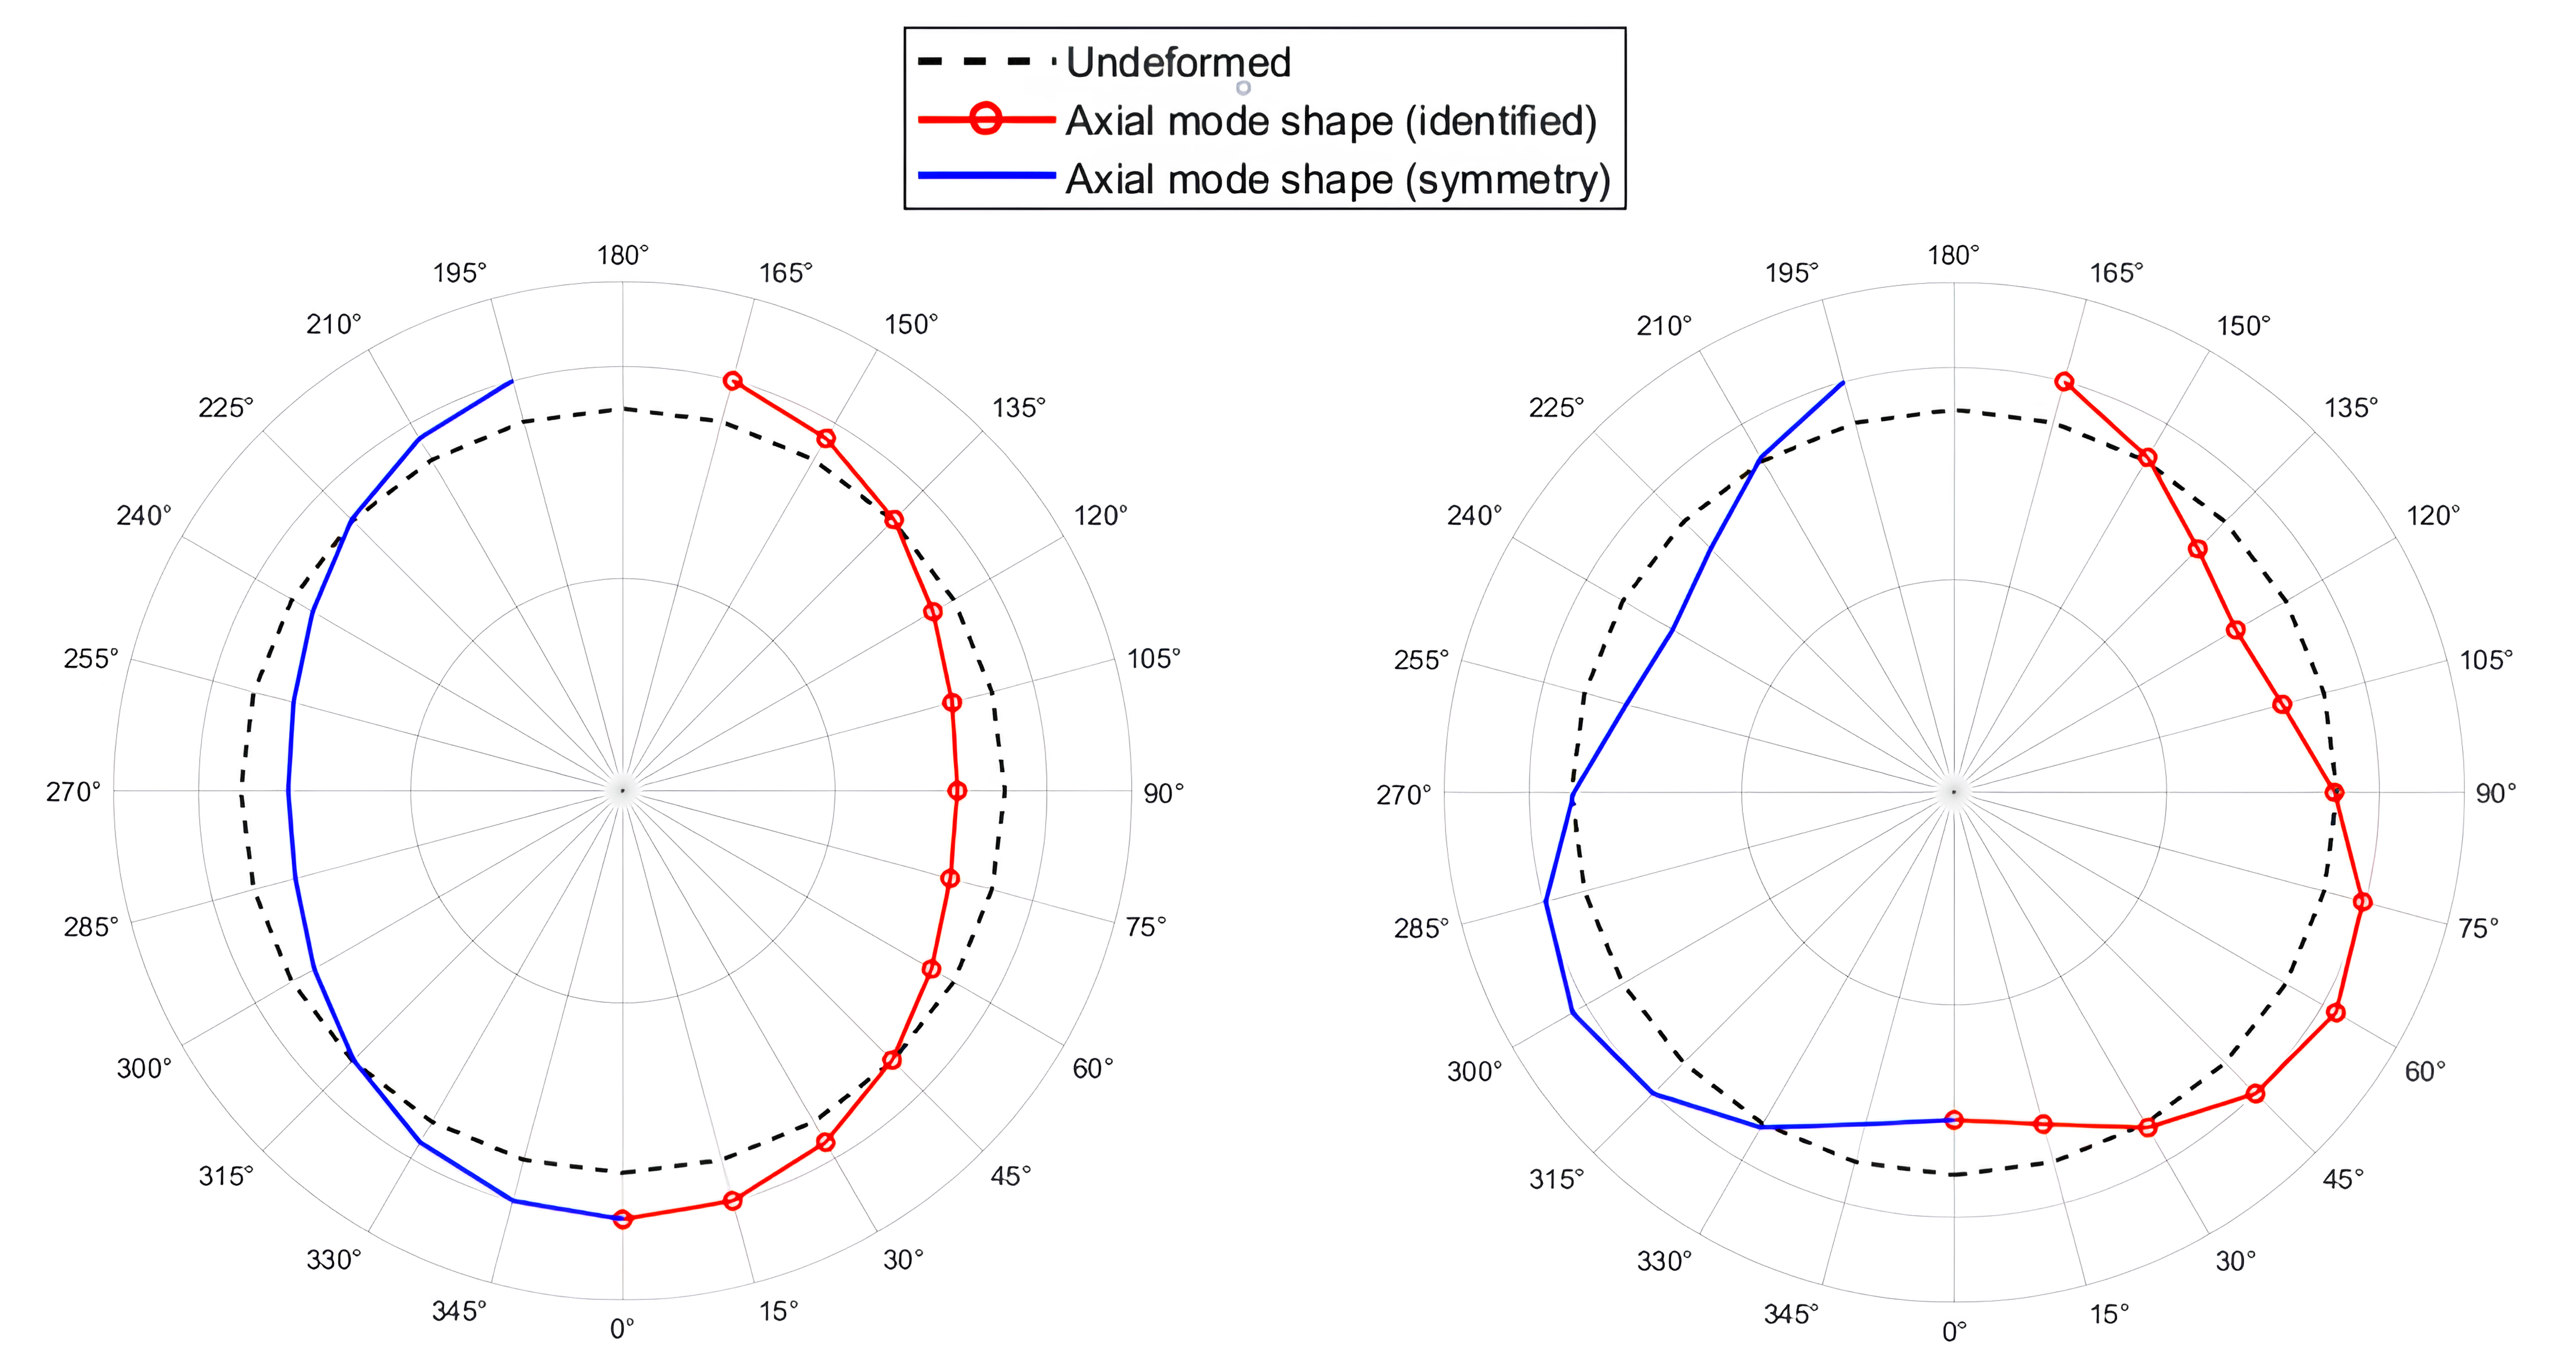
\includegraphics[scale=0.061]{Images/1 e 2 mode shapes.png}
    \caption{First and second axial mode shapes}
\end{figure}
\vspace{0.5cm}
\noindent Finally, the 12 points have been interpolated by means of a spline function, so that the curve is continuous to at least the second-order derivative at each point of the interval considered.\\
This provides a more realistic graphical representation of the physical phenomenon.\\
The interpolated mode shapes are reported below:
\begin{figure} [H]
    \centering
    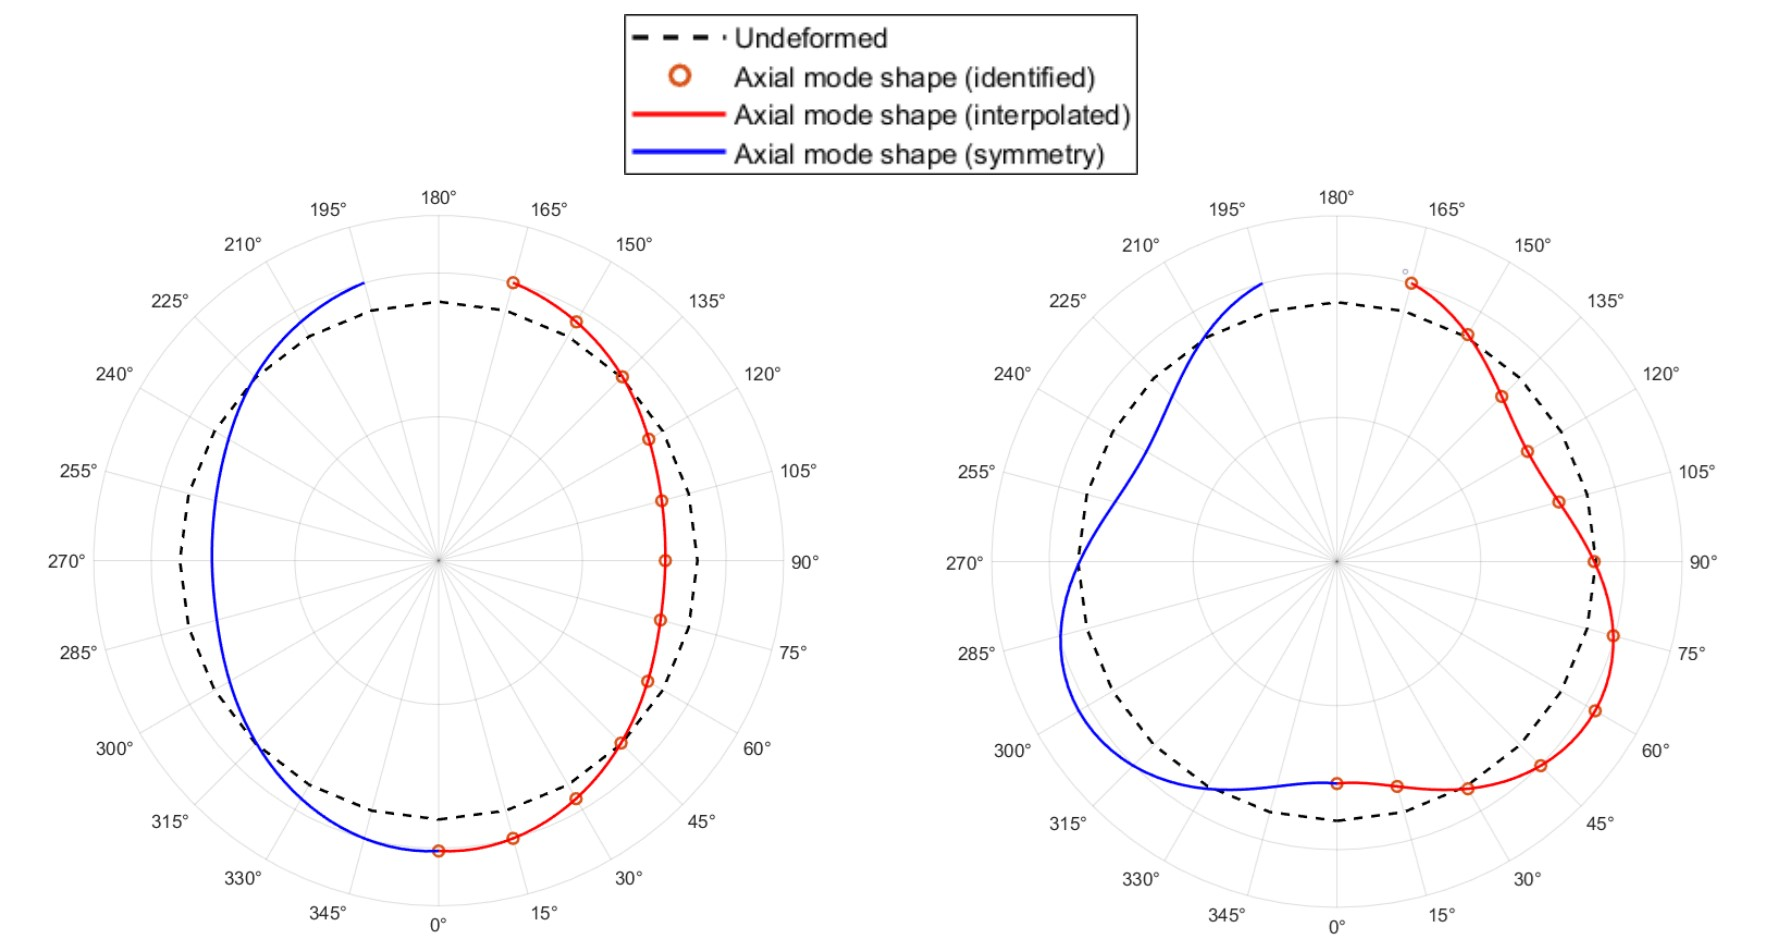
\includegraphics[scale=0.33]{Images/Interpolation.jpg}
    \caption{Interpolated first and second axial mode shapes}
\end{figure}






\newpage
% Creare una pagina vuota
\thispagestyle{empty} % Evita l'inserimento di intestazioni o piedini
\mbox{} % Inserisce uno spazio vuoto per creare una pagina vuota
\newpage

\thispagestyle{empty}
\addcontentsline{toc}{part}{Finite Element Analysis of an Harbour Crane}
\part*{Finite Element Analysis of an Harbour Crane}

\newcounter{Ass2}
\setcounter{Ass2}{0}
\renewcommand{\thesection}{\arabic{Ass2}}

\stepcounter{Ass2}
\section{Introduction}
\phantomsection
The second assignment consists of performing a Finite Element Analysis on a harbour crane made of steel beams.\\
More precisely, the aim of the first part is to derive the natural frequencies and the mode shapes of the structure.\\ 
The second one consists of employing the FE model to compute different frequency response functions for multiple input-output pairs and make a comparison with the ones obtained from the modal superimposition approach. \\
Finally the response of the structure has been computed when subjected to its own weight and to a moving load, simulating operating condition.\\

\stepcounter{Ass2}
\section{Finite Element Model}
\phantomsection

Firstly, a finite element (FE) model of the structure has been defined in a dedicated input file. \\
To achieve this, it has been computed the maximum element length based on the maximum frequency of interest (8 Hz), so to ensure that all elements operate in their quasi-static region within the examined bandwidth. \\
This condition is guaranteed by the following criteria, considering the lowest flexural stiffness and highest mass values (picked from the properties of the structure) and a safety factor equal to 2:


\begin{equation*}
    L < \sqrt{\frac{\pi^2}{{\eta\ \Omega_{max}}} \sqrt{\frac{EJ}{m}}} = 12.1 \text{ m}
\end{equation*}
\\
In order to have a more conservative approach, the elements employed have length between 6 m and 10 m. The obtained mesh is here reported:

\begin{figure}[H]
    \centering
    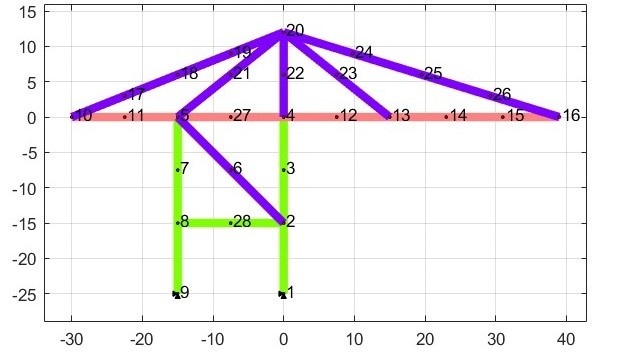
\includegraphics[scale=0.9]{figures/mesh.jpg}
    \caption{Undeformed structure and mesh}
\end{figure}


\stepcounter{Ass2}
\section{Natural frequencies and mode shapes}
\phantomsection

\noindent Once the mesh has been defined, the mass and stiffness matrices $\left[M\right]$ and $\left[K\right]$ have been assembled. This allowed to define the damping matrix $\left[C\right]$, according to the Rayleigh approach, as:
\begin{equation*}
    \left[C\right] = \alpha \left[M\right] + \beta \left[K\right]
\end{equation*}

\noindent with $\alpha = 0.1 \, s^{-1}$ and $\beta = 2.0 \times 10^{-4} \, s$.\\
\\
Subsequently, \(\left[M\right]\) and \(\left[K\right]\) have been partitioned into their free and constrained parts (\(\left[M_{FF}\right]\), \(\left[K_{FF}\right]\) and \(\left[M_{CC}\right]\), \(\left[K_{CC}\right]\) respectively).\\
This allowed to compute the natural frequencies and the modes (up to the third one) of the structure, indeed they're obtained solving the following eigenvalue and eigenvector problem:
\begin{equation*}
(\omega^2 [I] - [M_{FF}]^{-1} [K_{FF}])X = 0
\end{equation*}
The resulting natural frequencies are:
\begin{table}[H]
\centering
\renewcommand{\arraystretch}{1.4} % Imposta lo spazio tra le righe della tabella
\setlength{\tabcolsep}{13pt} % Imposta lo spazio tra le colonne della tabella
\begin{tabular}{|c|c|c|}
\hline
\multicolumn{3}{|c|}{\textbf{Natural frequencies}} \\
\hline
\nth{1} mode & \nth{2} mode & \nth{3} mode \\ \hline
0.98 Hz          & 2.53 Hz          & 3.57 Hz          \\ \hline
\end{tabular}
\caption{Natural frequencies}
\end{table}

\noindent The resulting mode shapes are:

\begin{figure} [H]
    \centering
    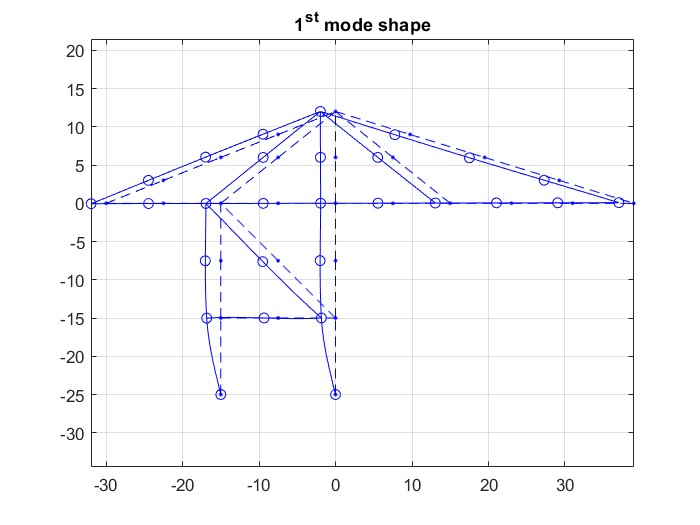
\includegraphics[scale=0.45]{figures/mode_1.jpg}
    \caption{First mode shape}
\end{figure}
\begin{figure} [H]
    \centering
    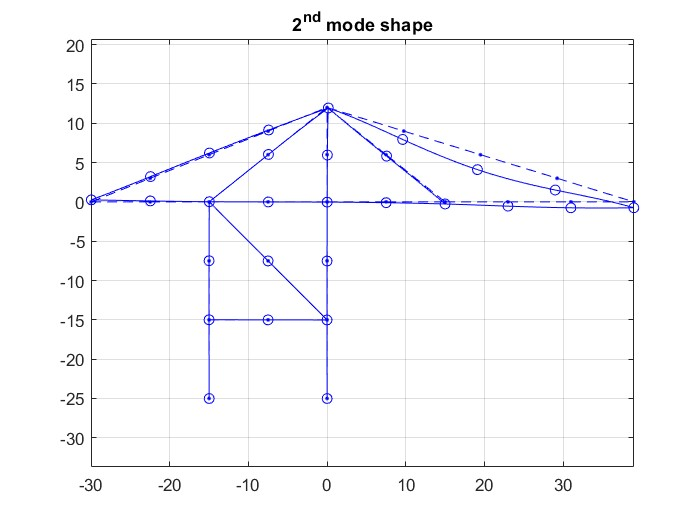
\includegraphics[scale=0.45]{figures/mode_2.jpg}
    \caption{Second mode shape}
\end{figure}
\begin{figure} [H]
    \centering
    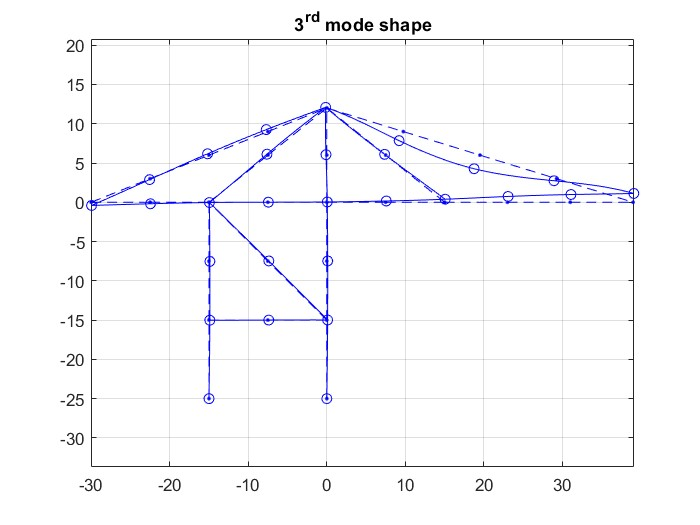
\includegraphics[scale=0.45]{figures/mode_3.jpg}
    \caption{Third mode shape}
\end{figure}
\noindent It is possible to notice that the shape of the plots depends on a chosen scale factor value (10 for the first mode, 3 for the second and third ones). 

\stepcounter{Ass2}
\section{Frequency response functions}
\phantomsection

\noindent Then two Frequency Response Functions (FRFs) have been computed, relating a vertical input force applied in point A with two different outputs: vertical displacement in point A and horizontal displacement in point B.\\
The FRFs have been obtained with the following:
\begin{equation*}
 \left[ H_{(input,output)} \right] = \left(-\Omega^2 \left[M_{FF} \right]+i\Omega \left[C_{FF} \right]+\left[K_{FF}\right] \right)^{-1}
\end{equation*}
Where: 
\begin{itemize}
    \item $\Omega$ is the vector containing the frequencies of interest (0$\div$8 Hz with resolution 0.01 Hz)
    \item $\left[M_{FF}\right]$, $\left[C_{FF}\right]$, $\left[K_{FF}\right]$  are the partitions of $[M]$, $[C]$ and $[K]$ related to the free nodes
\end{itemize} 
\ \\
\noindent ${F_{input}}$ is a vector having all the components equal to zeros except for the one corresponding to the degree of freedom in which the input force is applied (knowing the node in which the force is applied and its direction, we used the \textit{idb} matrix to compute the index of the non-null component).\\
$[H_{\text{input,output}}]$ is a matrix of size \textit{ndof} x \textit{length}($\Omega$) collecting all the transfer functions relating the input forces in ${F_{input}}$ with the displacements of the each free node.\\
Here \textit{idb} has been used again to specify the desired output displacements.\\
The two FRFs obtained are shown below.

    % \begin{figure}[H]
    % \centering
    % \makebox[\textwidth]{\hspace{-2cm}%posizione delle due immagini
    % \begin{minipage} {0.5\textwidth}
    %  
\includegraphics[scale=0.5]{Immagini report/FRFAA.jpg}
    %  \caption{FRF vertical force in A-vertical displacement in A}
    % \end{minipage}
    % \hspace{0.1\textwidth}%spazio tra le immagini
    % \begin{minipage} {0.5\textwidth}
    %  \begin{flushright}
    % 
\includegraphics[scale=0.5]{Immagini report/FRFAB.jpg}
    % \centering
    % \caption{FRF vertical force in A-vertical displacement in A}   
    %  \end{flushright}
    % \end{minipage}
    % }
    % \end{figure}

\begin{figure}[H]
\centering
\phantomsection\label{co-located TF}

\includegraphics[scale=0.75]{Immagini report/FRFAA.jpg}
\caption{FRF: vertical force in A - vertical displacement in A}
\end{figure}

\begin{figure}[H]
\centering
\phantomsection\label{Fig6}

\includegraphics[scale=0.75]{Immagini report/FRFAB.jpg}
\caption{FRF: vertical force in A - horizontal displacement in B}
\end{figure}


\noindent Firstly, looking at the co-located transfer function (\hyperref[co-located TF]{Figure 27}), it is possible to notice two clear resonance peaks in correspondence of the second and third eigenfrequencies, while for the first and fourth ones the function has a “flat” behaviour. \\
This happens since point A is located near a node of the structure regarding its vertical displacement for the first and fourth mode.\\
In \hyperref[Fig7]{Figure 29} the first four modes of the structure near point A are shown. \\
In the first and fourth mode point A does not move vertically, thus causing the cancellation of the corresponding resonance peaks.

\begin{figure} [H]
    \centering
    \phantomsection\label{Fig7}
    
\includegraphics[scale=0.39]{Immagini report/mode_shapes_ in_A_corretto.png}
    \caption{First four mode shapes in correspondence of point A}
\end{figure}

\noindent The second FRF (\hyperref[Fig6]{Figure 28}) relates the vertical force applied in A with the horizontal displacement in B.\\
It is interesting to notice that the module of the FRF is much lower both in terms of static and in-resonance displacement; this happens since the applied input force is vertical while the output displacement is horizontal.\\
As expected (considering the constraints), vertical and horizontal directions are quite decoupled.

\stepcounter{Ass2}
\section{Modal superposition approach}
\phantomsection

In this section it is computed the FRF relating the vertical input force applied in node A to the horizontal displacement in point B exploiting the modal superposition approach.\\
Considering the first two modes of the structure $\left[\phi\right]=\left[X_1,X_2\right]$, it is possible to compute the modal matrices:
\begin{equation*}
\left[M_m\right]=\left[\phi\right]^T\left[M_{FF}\right]\left[\phi\right] 
\end{equation*}
\begin{equation*}
\left[C_m\right]=\left[\phi\right]^T\left[C_{FF}\right]\left[\phi\right] 
\end{equation*}
\begin{equation*}
\left[K_m\right]=\left[\phi\right]^T\left[K_{FF}\right]\left[\phi\right] 
\end{equation*}
The dimension of all these matrices is equal to \textit{nmodes x nmodes}.\\
Then the Lagrangian component in modal coordinates can be expressed as: 
\begin{equation*}
    \left\{Q_m\right\}=\left[\phi\right]^T \left\{F_0\right\} \ \  \textit{(nmodes x 1)}
\end{equation*} 
Solving the equation of motion in modal coordinates we obtain:
\begin{equation*}
    \left\{q_0\right\}=\left(-\Omega^2\left[M_{m}\right]+i\Omega\left[C_{m}\right]+\left[K_{m}\right]\right)^{-1}\left\{Q_m\right\}
\end{equation*}
And transforming the coordinates back to the nodal ones, we obtain the FRF:
\begin{equation*}
   \left\{X_0\right\}=\left[\phi\right]\left\{q_0\right\} \quad
\rightarrow \quad
\left\{X_0\right\}=\left[\phi\right]\left(-\Omega^2\left[M_{FF}\right]+i\Omega\left[C_{FF}\right]+\left[K_{FF}\right]\right)^{-1}\left\{Q_m\right\}
\end{equation*}
Here is represented the FRF computed considering a unit input force:
\begin{figure} [H]
    \centering
    
\includegraphics[scale=0.75]{Immagini report/FRFAB_modfal.jpg}
    \caption{Comparison of FRF (vertical input in A, horizontal output in B) modal approach vs FE approach, considering the first 2 modes}
\end{figure}
 \ \\ 

\newpage

\noindent The FRF obtained using the modal superposition catches with a good approximation the resonance peaks corresponding to the modes used to compute the matrix $\left[\phi\right]$. \\
It is expected that increasing the number of modes leads to a better estimation of the FRF, since each mode would contribute to better approximate the real one.\\
However, choosing the length of the elements we are intrinsically imposing a constraint on the maximum reliable mode, in our case we can obtain coherent results only up to 8 Hz.
\ \\
\begin{figure} [H]
    \centering
    
\includegraphics[scale=0.75]{Immagini report/FRFAB_modfal_con3 modes.jpg}
    \caption{Comparison of FRF modal approach vs. FEM approach considering the first 3 modes}
\end{figure}

\noindent Considering three modes it is possible to describe much better the behaviour of the FRF, especially around the third mode.\\
Thus, if the analysis is focused on the behaviour of the structure in a certain frequency range, thanks to the modal superposition approach it is possible to obtain quite a good approximation of the FRF considering the modes close to that range.

\stepcounter{Ass2}
\section{FRF in the constraint}
\phantomsection

It has been obtained the FRF relating the input force applied at point C in vertical direction to the output axial force in the right column evaluated at point O$_2$.\\
The vector of the reaction forces  can be computed as:

\begin{equation*}
    \left\{x_F\right\}=\{ X_0 \}\ e^{\left\{i\Omega t\right\}}
\end{equation*}
\begin{equation*}
   \{ X_0 \} =\left.\ \left(-\Omega^2\left[M_{FF}\right]+ i\ \Omega\left[C_{FF}\right]+ \left[K_{FF}\right]\right.\right)^{-1}\{F_0\}\ 
\end{equation*}
\begin{equation*}
    \{ R_0 \}=\left.\ \left( -\Omega^2\left[M_{CF}\right]+i\ \Omega\left[C_{CF}\right]+\left[K_{CF}\right]\right.\right)^{-1}\{ X_0 \}
\end{equation*}

Where:
\begin{itemize} 
    \item $\{F_0\}$ is a vector which is null everywhere except for a one in the position corresponding to the vertical force in C
    \item $[M_{CF}], [C_{CF}], [K_{CF}]$ are the partitions of $[M], [C]$, and $[K]$ respectively, relating the constrained nodes with  the free nodes
    \item $\left\{X_0\right\}$ is the response of the free nodes in terms of displacement due to the input $\left\{F_0\right\}$
    \item $\left\{R_0\right\}$ is the vector of reaction forces at the constrained nodes
\end{itemize}
The FRF below is computed from the {R} vector, extracting the element corresponding to the vertical force in O$_2$.
\begin{figure} [H]
    \centering
    
\includegraphics[scale=0.75]{Immagini report/FRFCO2.jpg}
    \caption{FRF vertical force in C - vertical reaction force in O_2}
\end{figure}
\noindent This transfer function has a higher modulus mainly for two reasons: firstly, it relates the input force to an output being a force as well, thus the FRF is non dimensional.\\
Secondly, the reaction force in O$_2$ is expected to sustain a large part of the input force, since the structure is grounded in two points only.

\stepcounter{Ass2}
\section{Static response}
\phantomsection

The static response of the structure is obtained applying to each element a distributed load equal to its mass per unit length.\\
Moving to the local reference, it is possible to compute the nodal forces acting on each element by imposing a forces and moments equilibrium.\\By summing the nodal forces and moving back to the global reference frame it is possible to compute the deflection.
\begin{equation*}
    \{F\}^{\{L\}}_{k} =
    \begin{bmatrix}
    \frac{L_k}{2} & 0 \\
    0 & \frac{L_k}{2} \\
    0 & -\frac{{L_k}^2}{12} \\
    \frac{L_k}{2} & 0 \\
    0 & \frac{L_k}{2} \\
    0 & -\frac{{L_k}^2}{12} 
    \end{bmatrix}
    \left\{
\begin{array}{c}
p_{0x}^{(L)} \\
p_{0y}^{(L)}
\end{array}
\right\}\ \ \ \ \ \ 
\{F\}^{\{G\}}_{k} = [\Lambda_k] \{F\}^{\{L\}}_{k}
    {\ \ \ \ \ \ \left\{F\right\}}^{\left\{G\right\}}=\sum_{k}{\left.\left[E_k\right.\right]\left\{F\right\}_k^{\left\{G\right\}}}
\end{equation*}
Once the vector of the nodal forces in the global reference has been obtained, the displacement is computed with the following:\\
\begin{equation*}
 \left\{X_{st}\right\}=\left[K_{FF}\right]^{-1}\left\{F\right\}^{\left\{G\right\}}   
\end{equation*}

\begin{figure} [H]
    \centering
    \phantomsection\label{Staticresponse}
    
\includegraphics[scale=0.6]{Immagini report/static deflection.jpg}
    \caption{Static deflection due to the weight of the entire structure}
\end{figure}
\noindent In \hyperref[Staticresponse]{Figure 33} it is possible to observe the static response of the structure due to its weight. The maximum static deflection is 53.6 mm(vertical component -53.1 mm, horizontal component -7.5 mm) and is reached in node 25.

\newpage

\stepcounter{Ass2}
\section{Moving load}
\phantomsection

In this section the behavior of the structure with a load moving from point D to A is analysed.\\
It starts with zero initial velocity, uniformly accelerates over the first 8 meters, keeps a constant velocity over the next 8 meters and then decelerates until reaching point A with null velocity.\\
Knowing the total travel time (20 s), it is possible to compute the velocity profile which satisfies all the constraints:
\vspace{0.3 cm}
\begin{figure} [H]
    \centering
    
\includegraphics[scale=0.55]{Immagini report/velocity_profile.jpg}
    \caption{Velocity profile of the load's motion}
\end{figure}
\noindent Knowing the velocity profile, the motion can be divided in discrete time intervals, computing for each time step the position of the load \(\overline{x}\), which results to be: \( \overline{x}(t) = vt \) \\
The Lagrangian components are computed as:

\begin{equation*}
\left\{
\begin{aligned}
    &\delta L = \delta w(\overline{x})F_0  \\
    &\delta w(\overline{x}) = \underline{\phi} (\overline{x})^T
    \delta \underline{q}
\end{aligned}
\right. \quad \Rightarrow \quad 
\delta L = \delta \underline{q}^T \underline{\phi} (\overline{x}) F_0
\end{equation*}

\begin{equation*}
\delta L = \delta \underline{q}^T \underline{Q}(t)
\quad \Rightarrow \quad 
\underline{Q}(t) = \underline{\phi} (\overline{x}) F_0 = \underline{\phi} (vt) F_0
\end{equation*}
Once \(\underline{Q}(t)\) is known, it has been possible to solve the resulting set of ODEs obtaining the modal coordinates \(\overline{q}\)(t) in each time instant. \\
Finally it has been possible to reconstruct the time history of the vertical displacement of point A as follows:
\begin{equation*}
    w_A = \left[ \phi (x_A) \right] \overline{q}(t)
\end{equation*}
In the following it has been plotted the resulting time history:

\begin{figure} [H]
    \centering
    
\includegraphics[scale=0.5]{Immagini report/Andamento.jpg}
    \caption{Time history of the vertical displacement in point A due to a moving load of 1000N}
\end{figure}

\end{document}